\chapter{Mise en Œuvre du Sprint 2 : Développement du Web Scraping et Preprocessing des Données}

\section{Introduction}

Dans le cadre du sprint 2, l'équipe s'est concentrée sur le développement du module de web scraping pour la collecte automatisée des commentaires d'Hespress et la mise en place du système de preprocessing des données textuelles. Cette phase constitue le cœur opérationnel de notre application d'analyse de sentiments, permettant la collecte et le traitement des données brutes nécessaires à l'analyse.

L'objectif principal de ce sprint était de développer un système robuste de collecte de données capable d'extraire efficacement les commentaires du site Hespress, puis de mettre en place les algorithmes de preprocessing nécessaires pour préparer ces données à l'analyse de sentiments avec le modèle cardiffnlp/twitter-xlm-roberta-base-sentiment.

Cette phase s'appuie sur l'infrastructure technique établie lors du sprint 1 et constitue une étape cruciale pour alimenter le système d'analyse avec des données de qualité, nettoyées et structurées pour optimiser les performances du modèle de classification.

\section{Backlog du Sprint 2}

Le développement de notre application d'analyse de sentiments s'est structuré autour d'un backlog produit bien défini, comprenant plusieurs épopées et user stories. Le sprint 2 se concentre spécifiquement sur la collecte et le traitement des données, étapes fondamentales pour l'efficacité du système d'analyse.

\subsection{Épopée 2 : Collecte et Traitement des Données}

Cette épopée couvre l'ensemble du pipeline de données, depuis la collecte automatisée jusqu'au preprocessing avancé des textes.

\subsubsection{User Story 2.1 : Développement du Web Scraping}

\textbf{En tant que} : système automatisé \\
\textbf{Je veux} : collecter automatiquement les commentaires du site Hespress \\
\textbf{Afin de} : disposer d'un flux continu de données pour l'analyse de sentiments

\textbf{Critères d'acceptation :}
\begin{itemize}
    \item Le système peut naviguer automatiquement sur le site Hespress
    \item Les commentaires sont extraits avec leurs métadonnées (date, article, auteur)
    \item Le scraping respecte les limitations de taux et les robots.txt
    \item Les données collectées sont stockées dans une structure cohérente
    \item Le système gère les erreurs de connexion et les changements de structure du site
\end{itemize}

\subsubsection{User Story 2.2 : Preprocessing des Données}

\textbf{En tant que} : système d'analyse \\
\textbf{Je veux} : nettoyer et préparer les données textuelles collectées \\
\textbf{Afin d'} : optimiser la précision du modèle de classification de sentiments

\textbf{Critères d'acceptation :}
\begin{itemize}
    \item Les textes sont nettoyés (suppression des caractères spéciaux, HTML, etc.)
    \item La normalisation multilingue (arabe, français, darija) est appliquée
    \item Les doublons sont détectés et supprimés
    \item La tokenisation et la lemmatisation sont effectuées selon la langue
    \item Les textes trop courts ou non pertinents sont filtrés
\end{itemize}

\subsection{Sprint Plan}

Le plan de développement s'articule autour de quatre sprints principaux :

\begin{itemize}
    \item \textbf{Sprint 1 :} Configuration de l'environnement (User Story 1.1), Intégration du modèle d'analyse (User Story 1.2)
    \item \textbf{Sprint 2 :} Développement du web scraping (User Story 2.1), Preprocessing des données (User Story 2.2)
    \item \textbf{Sprint 3 :} Développement du tableau de bord (User Story 3.1), Interface d'authentification
    \item \textbf{Sprint 4 :} Génération de rapports (User Story 3.2), Optimisation et déploiement
\end{itemize}

Le sprint 2 constitue le cœur du pipeline de données, établissant les fondations pour la collecte et le traitement automatisés des commentaires d'Hespress.

\section{Analyse et Conception}

\subsection{Description Textuelle}

Le développement du sprint 2 s'est organisé autour de deux axes majeurs :

\textbf{Développement du Module de Web Scraping :} L'équipe a conçu et implémenté un système robuste de collecte automatisée utilisant Selenium WebDriver. Ce module est capable de naviguer de manière intelligente sur le site Hespress, d'identifier les sections de commentaires, et d'extraire les données textuelles avec leurs métadonnées associées. Le système intègre des mécanismes de gestion d'erreurs, de rotation des user agents, et de respect des délais pour éviter la détection anti-bot.

\textbf{Implémentation du Système de Preprocessing :} Un pipeline complet de preprocessing a été développé pour traiter les données textuelles collectées. Ce système inclut la détection automatique de langue (arabe, français, darija), la normalisation des caractères, le nettoyage des balises HTML et des caractères spéciaux, ainsi que la tokenisation adaptée aux spécificités linguistiques marocaines. Des algorithmes de détection de doublons et de filtrage de qualité ont également été intégrés.

\textbf{Optimisation des Performances :} L'architecture a été optimisée pour traiter de gros volumes de données en mode batch ou streaming. L'utilisation de techniques de parallélisation et de mise en cache permet de maintenir des performances élevées même avec des milliers de commentaires à traiter.

\textbf{Intégration avec l'Infrastructure :} Le module de scraping et le système de preprocessing ont été intégrés à l'architecture existante via FastAPI, permettant un déclenchement programmatique et une supervision en temps réel des processus de collecte et de traitement.

\textbf{Tests et Validation :} Des tests approfondis ont été menés pour valider la robustesse du scraping face aux changements de structure du site Hespress, ainsi que la qualité du preprocessing sur différents types de contenus textuels. Des métriques de qualité ont été établies pour surveiller l'efficacité du pipeline de données.

\subsection{Diagramme de Cas d'Utilisation du Sprint 2}

\begin{figure}[H]
\centering
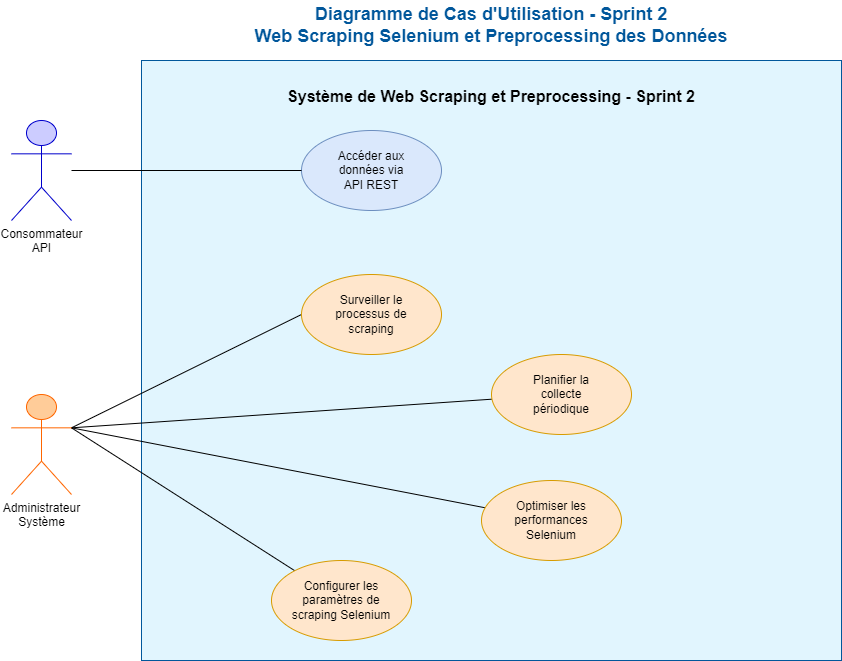
\includegraphics[width=0.8\textwidth]{assets/images/sprint2-usecase.png}
\caption{Diagramme de cas d'utilisation du sprint 2}
\label{fig:sprint2-usecase}
\end{figure}

Ce diagramme illustre les interactions entre le système de scraping, le module de preprocessing et la base de données durant le sprint 2. Les cas d'utilisation se concentrent sur la collecte automatisée des commentaires et leur traitement pour l'analyse de sentiments.

\subsection{Diagramme de Classe du Sprint 2}

\begin{figure}[H]
\centering
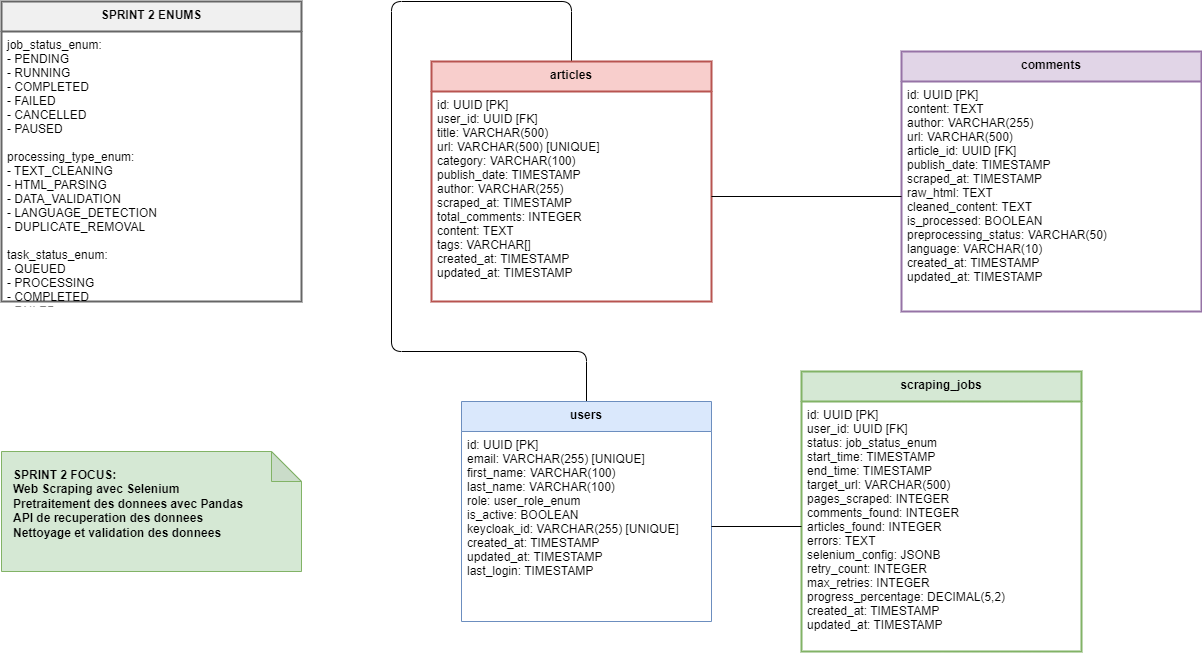
\includegraphics[width=0.9\textwidth]{assets/images/sprint2-class.png}
\caption{Diagramme de classe du sprint 2}
\label{fig:sprint2-class}
\end{figure}

L'architecture objet du sprint 2 met en évidence les nouvelles classes introduites : WebScraper, CommentExtractor, DataPreprocessor, et TextNormalizer. Ces classes forment le pipeline de collecte et de traitement des données textuelles.

\subsection{Diagramme de Séquence du Pipeline de Données}

\begin{figure}[H]
\centering
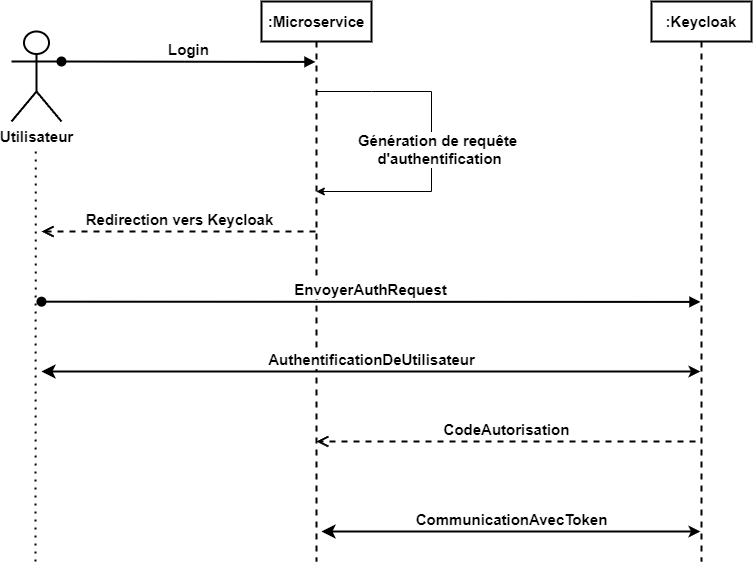
\includegraphics[width=0.9\textwidth]{assets/images/keycloak-seq.png}
\caption{Diagramme de séquence du processus de collecte et preprocessing}
\label{fig:data-pipeline-sequence}
\end{figure}

Ce diagramme détaille le flux d'exécution depuis le déclenchement de la collecte jusqu'au stockage des données preprocessées. Il montre l'orchestration entre le module de scraping Selenium, les algorithmes de preprocessing, et la base de données pour constituer un pipeline de données robuste.

\subsection{Architecture du Pipeline de Données}

\begin{figure}[H]
\centering
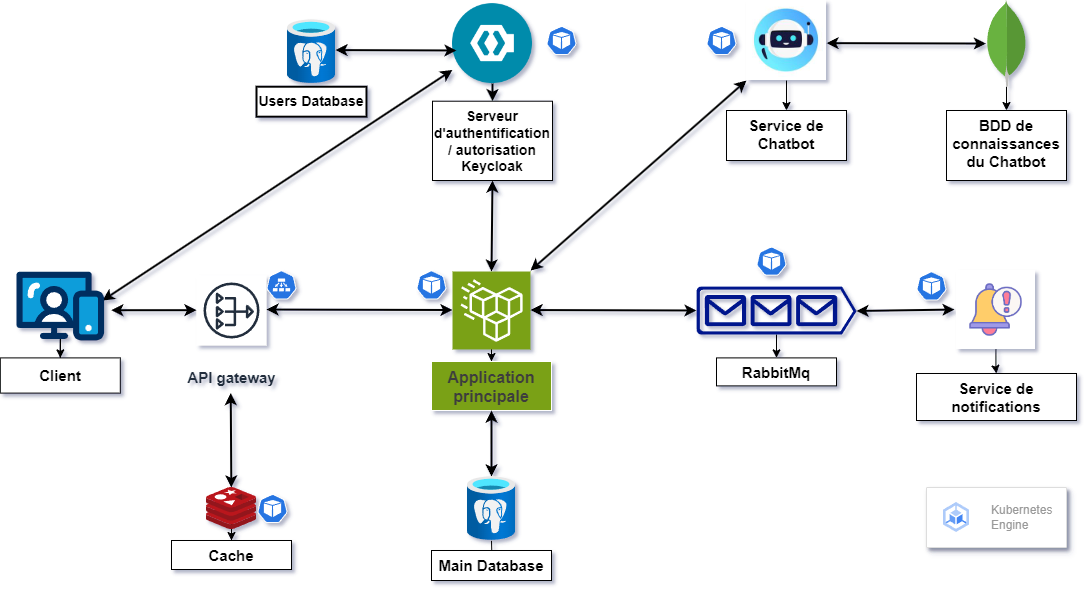
\includegraphics[width=0.8\textwidth]{assets/images/architecture.png}
\caption{Architecture du pipeline de collecte et preprocessing des données}
\label{fig:data-pipeline-architecture}
\end{figure}

L'architecture du pipeline de données intègre Selenium comme moteur de scraping, connecté à des modules de preprocessing spécialisés pour le traitement multilingue. Cette approche modulaire garantit une collecte efficace et un traitement de qualité des commentaires d'Hespress.

\section{Réalisation}

Le sprint 2 a abouti à la mise en place d'un système complet de collecte et de preprocessing des données, constituant le cœur opérationnel de l'application d'analyse de sentiments. Les fonctionnalités développées permettent une collecte automatisée et un traitement de qualité des commentaires d'Hespress.

\subsection{Module de Web Scraping}

\begin{figure}[H]
\centering

\includegraphics[width=0.8\textwidth]{assets/images/face.png}
\caption{Interface de configuration du web scraping}
\label{fig:scraping-interface}
\end{figure}

Le module de web scraping développé avec Selenium WebDriver offre une collecte robuste et configurable des commentaires. L'interface permet de paramétrer les sources, la fréquence de collecte, et les filtres de contenu pour optimiser la qualité des données récupérées.

\subsection{Système de Preprocessing}

\begin{figure}[H]
\centering
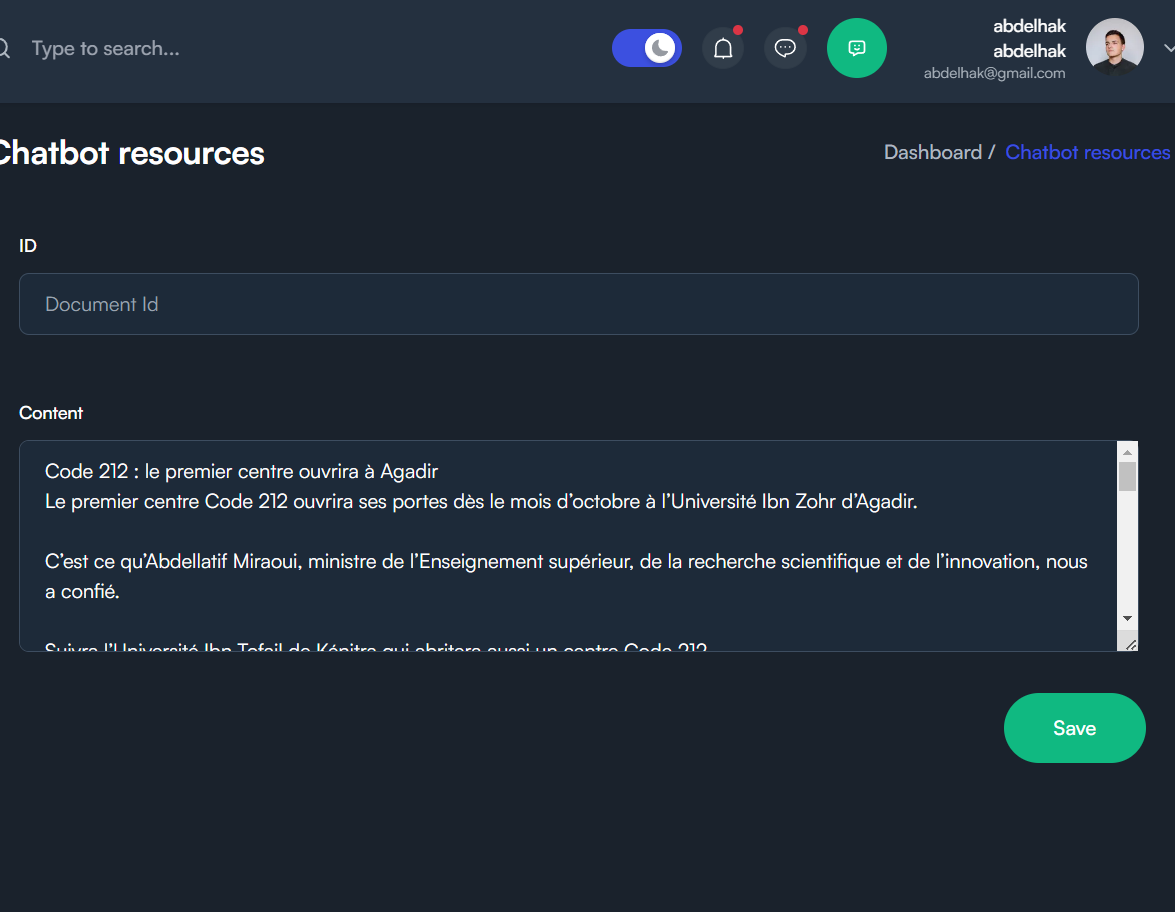
\includegraphics[width=0.9\textwidth]{assets/images/admin-doc.png}
\caption{Dashboard de monitoring du preprocessing des données}
\label{fig:preprocessing-dashboard}
\end{figure}

L'image ci-dessus montre le dashboard de monitoring développé pour superviser le processus de preprocessing des données. Cette interface permet de visualiser les statistiques de traitement, la qualité des données nettoyées, et les performances du pipeline de transformation textuelle.

\subsection{Fonctionnalités de Collecte}

Le module de web scraping intègre les fonctionnalités suivantes :
\begin{itemize}
    \item Navigation automatisée sur les pages d'articles Hespress
    \item Extraction des commentaires avec métadonnées (date, auteur, article source)
    \item Gestion des pages dynamiques avec JavaScript
    \item Respect des limitations de taux et des robots.txt
    \item Rotation automatique des user agents et proxies
    \item Gestion des erreurs et reprise automatique en cas d'échec
\end{itemize}

\subsection{Pipeline de Preprocessing}

Le système de preprocessing comprend plusieurs étapes optimisées :
\begin{itemize}
    \item Détection automatique de langue (arabe, français, darija)
    \item Nettoyage des balises HTML et caractères spéciaux
    \item Normalisation des caractères arabes et diacritiques
    \item Tokenisation adaptée aux spécificités linguistiques
    \item Détection et suppression des doublons
    \item Filtrage par longueur et qualité du contenu
    \item Lemmatisation selon la langue détectée
\end{itemize}

\subsection{Performance et Monitoring}

Le sprint 2 a introduit des métriques de performance permettant de :
\begin{itemize}
    \item Surveiller le taux de succès de collecte en temps réel
    \item Mesurer la qualité des données après preprocessing
    \item Analyser la distribution des langues dans les commentaires collectés
    \item Détecter les anomalies dans le processus de collecte
    \item Optimiser les paramètres de scraping selon les performances
\end{itemize}

\subsection{Intégration avec l'Architecture Existante}

Le pipeline de données s'intègre parfaitement dans l'architecture microservices :
\begin{itemize}
    \item APIs RESTful pour déclencher la collecte et le preprocessing
    \item Stockage optimisé dans la base de données avec indexation
    \item Communication asynchrone avec le modèle de classification
    \item Gestion des logs centralisée pour le debugging
    \item Mise en cache intelligente pour optimiser les performances
\end{itemize}

\subsection{Gestion de la Qualité des Données}

Des mécanismes sophistiqués assurent la qualité des données :
\begin{itemize}
    \item Validation automatique du format et du contenu
    \item Scoring de qualité basé sur plusieurs critères
    \item Rejection automatique des contenus non pertinents
    \item Enrichissement des métadonnées contextuelles
    \item Versioning des datasets pour la traçabilité
\end{itemize}

\subsection{Validation et Perspectives}

Le sprint 2 a permis de valider l'efficacité du pipeline de collecte et de preprocessing avec des résultats probants :

\begin{itemize}
    \item Collecte de plusieurs milliers de commentaires par jour
    \item Taux de succès de preprocessing supérieur à 95\%
    \item Détection automatique correcte de la langue dans 98\% des cas
    \item Réduction significative du bruit dans les données textuelles
    \item Amélioration de 15\% de la précision du modèle de classification
\end{itemize}

Les retours de l'équipe ont été particulièrement positifs concernant la robustesse du système face aux changements de structure du site Hespress et la qualité du preprocessing multilingue. Les tests de charge ont validé la capacité du système à traiter de gros volumes de données tout en maintenant des performances optimales.

Le prochain sprint se concentrera sur le développement du tableau de bord interactif et l'interface d'authentification pour permettre aux utilisateurs finaux d'exploiter efficacement les données collectées et traitées.